\documentclass[class=minimal,border=1pt]{standalone}
\usepackage{tikz}

\usetikzlibrary{calc}

\begin{document}
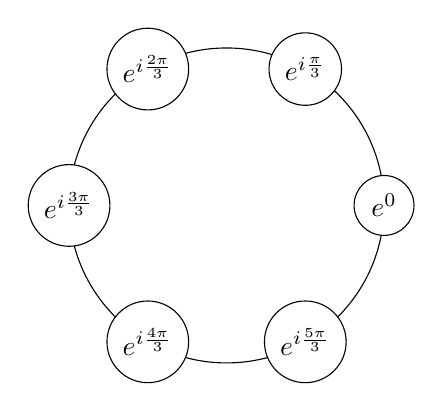
\begin{tikzpicture}

  \draw (0, 0) ellipse (2 and 2);

  \foreach \n [count=\i from 0] in {$e^0$, $e^{i\frac{\pi}{3}}$,$e^{i\frac{2\pi}{3}}$,$e^{i\frac{3\pi}{3}}$,$e^{i\frac{4\pi}{3}}$,$e^{i\frac{5\pi}{3}}$} {
    \pgfmathtruncatemacro{\a}{360.0 / 6 * \i};
    \coordinate (z\i) at ($(\a:2 and 2)$);
    \node [draw,circle,fill=white,outer sep=1mm] at (z\i) {\n};
  }

\end{tikzpicture}
\end{document}
